\subsection{Preprocesamiento De Los Datos} 
Con el objetivo de darle mayor estabilidad matematica a los datos y quitar algo del ruido que puedan tener, realizamos un preprocesamiento de los mismos. El mismo consistió en quitar los utliers dentro del set de datos y luego normalizarlos con media 0 y varianza 1.

\subsection{Implementacion Del algoritmo} 

El algoritmo que implementamos consistió en una red neuronal profunda con retropropagación del error. Este, descripto de manera informal consiste en introducir una instancia del problema, calcular la salida, compararla con la salida esperada y retropropagar el error, con el objetivo modificar las matrices de pesos y minimizar la diferencia. El sistema implementado se dice ser $online$ ya que los pesos de las matrices son ajutados luego de retropropagar el error de cada instancia en vez de hacerlo al final de la epoca.

A fin de tener una medida de como va \"aprendiendo\" la red neuronal, luego de presentarle a la red todas las instancias una vez, calculamos la norma de la diferencia entre las respuestas obtenidas y las esperadas. Consideraremos esta nuestra "norma del error" y la tomaremos como una metrica adecuada para saber cuan buenos resultados devuelve nuestra red.

%habria que poner pseudocodigo o algo mas lindo acá
%Aprovechando este calculo de la norma, decidimos agregar a la implementación, un learning rate adaptativo. El mismo consiste en, en caso de que la norma haya decrecido, aumentar el learnin rate. En caso contrario, es decir, la norma del error aumentó, quiere decir que la red empeoro la solucion y decrecemos el learnig rate.

%falta explicar un poco mejor las funciones de activacion que usamos, etc

Como optimización adicional se agrego un termino de momentum. La idea tras esto consiste en darle a cada peso de la matriz una "inercia" que le permita continuar avanzando en la direccion en la que avanzó en la iteración anterior. El objetivo consiste en disminuir las oscilaciones con cada pequeño cambio en la matriz.

\subsection{Experimentación sobre datos de Diagnostico de Cancer}

\subsubsection{Convergencia del algoritmo} 

Para este problema utilizaremos una neurona en la ulima capa con función de activación logistica. Para ser consistentes con esto, las salidas esperadas adoptarán los valores $1$ si resulto ser cancer maligno, y $0$ si resulto ser benigno. La experimentación consistirá en buscar los parametros optimos que nos den la mayor tasa de aciertos para nuestro data set.

Como primera instancia comprobaremos que la red converge efectivamente a la solución esperada. Para eso tomamos un lerning rate de $0.01$ y con $1300$ epocas graficamos la norma del error cada $1000$ iteraciones:

\begin{figure}[h!]
  \centering
    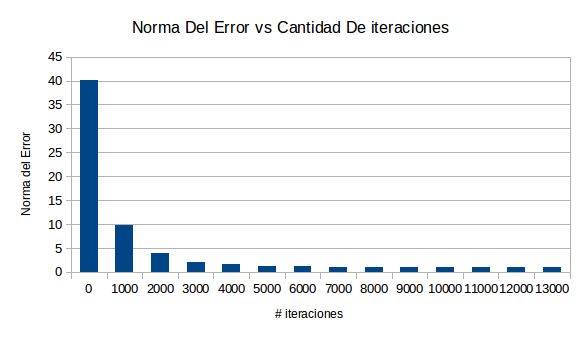
\includegraphics[scale=0.4]{ej1_convergencia/1.png}
\end{figure}

El grafico muestra que, efectivamente, nuestro algoritmo minimiza la diferencia entre las soluciones obtenidas y las deseadas, minimizando así tambien la norma del error.

\subsubsection{Performance Vs Learning Rate} 

%Capaz va mas arriba?
Para evitar el sobreajuste las experimentaciones todas las experimentaciones desde este punto se realizarán con la siguente metodología. Se dividirá el set de datos de entrenamiento provisto por la catedra en dos sets de datos distintos. Uno se utilizará para entrenar la red, mientras que el otro se medirán que tan buenos fueron los resultados obtenidos. Con esto se espera reducir el overfittning que la red pueda generar y comprobar de manera mas acertada que tan buenos resultados dará la red sobre datos reales del problema.

Ademas, para visualizar los resultados mas claramente utilizaremos una matriz de confución, que nos permitirá dicernir entre falsos positivos (fp), falsos negativos(fn) y instancias clasificadas correctamente (tp y tn).

\reescribir 

En esta sección querremos experimentar es como se comporta el algoritmo al variar el learning rate. Para ello, dejamos constantes las cantidad de epocas de entrenamiento en $10000$ y variamos el learning desde $0.01$ hasta $0.2$ aumentando de a $0.01$

\begin{figure}[h!]
\centering
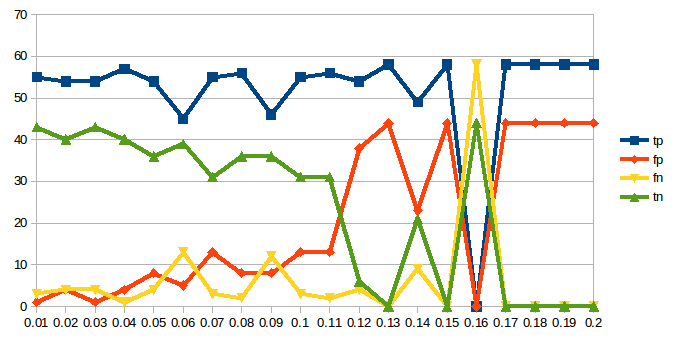
\includegraphics[scale=0.4]{ej1_test_learning_rate/1.png}
\end{figure}

El grafico muestra varios resultados interesantes. En el rango $[0.01,0.11]$ puede verse que la red arroja buenos resultados, obteniendo en general un $90\%$ de clasificaciones corrrectas. Pasado ese rango puede verse como los falsos positivos y los falsos negativos sufren un incremento muy significativo, llegando al final a casi un $50\%$ de clasificaiones incorrectas. Consideramos que para estos casos la red neuronal divergió, posiblemente debido a que multiplicar el gradiente por un valor muy grande lleva a "pasarnos" del minimo y por lo tanto reduciendo la precición del algoritmo. \completar

\subsubsection{Performance Vs Cantidad De iteraciónes} 

Como siguiete paso buscaremos analizar el comportamiento de la red para distintas cantidades de iteraciones, viendo si existe algun cambio significativo en este sentido. Para ello dejamos fijo el learning rate fijo en $0.01$ ya que consideramos que este nos da los resultados mas aceptables y variamos la cantidad de iteraciones.

\begin{figure}[h!]
  \centering
    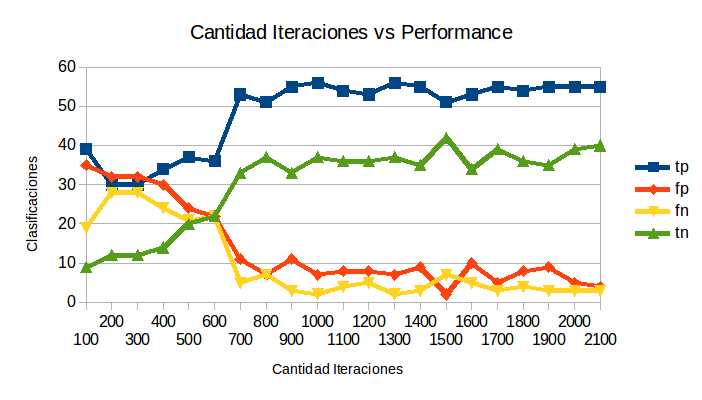
\includegraphics[scale=0.4]{ej1_test_iter/1.png}
\end{figure}

Para una cantidad menor a $600$ iteraciones puede observarse que la red neuronal tiene una performance mala obteniendo un porcentaje de falsos negativos y falsos positivos cercano al $50\%$. Ya con $700$ iteraciones en adelante la performance del algoritmo mejora drasticamente, rondando el porcentaje de falsos negativos y falsos positivos al rededor de $10 \%$ y $20\%$. Para $2000$ y $2100$ iteraciones obtenemos un $7\%$  de falsos negativos.


\subsection{Eficiencia energética} 

%explicar modificacion?

De igual manera realizamos la misma experimentación para este problema de regreción lineal. Como primera instancia queremos ver si el algoritmo converge adecuadamente para este problema.

\begin{figure}[h!]
  \centering
    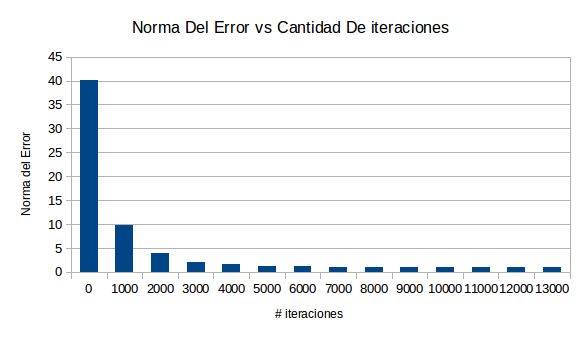
\includegraphics[scale=0.4]{ej1_convergencia/1.png}
\end{figure}